\documentclass[xcolor=svgnames,dvipsnames,table, hyperref=pdftex, mathserif, presentation]{beamer}
\usepackage{amsmath,amssymb,amsfonts,amsthm}
\usepackage{ctex}
\setCJKsansfont{KaiTi}% 文泉驿的黑体
\usepackage{graphics}
\usepackage{graphicx}
\usepackage{xcolor}
\usepackage{wasysym}
\usepackage{bbm}
\usepackage{url}
\usepackage{beamerleanprogress}
\usepackage{tikz-dependency}
\usepackage{tikz-qtree}
\usepackage{multirow}


% for uml charts
\usepackage{tikz}
\usetikzlibrary{calc,arrows.meta, graphs, trees, shapes, positioning, automata,
shapes.geometric, shapes.multipart, er, patterns, decorations.markings, intersections, decorations.text}
\usepackage{tikz-uml}

% for overlap pictures
\usepackage{overpic}

% 为了插入c代码
\usepackage{listings}



% for customize itemize
% \usepackage{lipsum}
% \usepackage{paralist}
% \setbeamertemplate{itemize/enumerate body begin}{\large}
% \setbeamertemplate{itemize/enumerate subbody begin}{\tiny}


\newcommand{\tabincell}[2]{\begin{tabular}{@{}#1@{}}#2\end{tabular}}%放在导言区
\usetheme{CambridgeUS}
%\usetheme{Pittsburgh}
\usecolortheme{orchid} % seahorse  orchid rose
\setbeamertemplate{blocks}[rounded][shadow=true]
\AtBeginSection[]{%
  \begin{frame}<beamer>
    \frametitle{Outline}
      \tableofcontents[current] 
    \end{frame}
  \addtocounter{framenumber}{-1}% If you don't want them to affect the slide number
}
\AtBeginSubsection[]
{
  \begin{frame}
  \frametitle{Outline}
    \tableofcontents[currentsection,currentsubsection]
  %\tableofcontents[sectionstyle=show/hide,subsectionstyle=hide/show/hide]
  \end{frame}
  \addtocounter{framenumber}{-1}% If you don't want them to affect the slide number
}
\newcommand{\setof}[1]{\ensuremath{\left \{ #1 \right \}}}
\newcommand{\tuple}[1]{\ensuremath{\left \langle #1 \right \rangle }}
\newcommand{\red}[1]{\textcolor{red}{#1}}
\newcommand{\brown}[1]{\textcolor{brown}{#1}}
\newcommand{\green}[1]{\textcolor{green}{#1}}
\newcommand{\blue}[1]{\textcolor{blue}{#1}}
\newcommand{\cyan}[1]{\textcolor{cyan}{#1}}
\newcommand{\cCode}[0]{\lstset{language=C++,
                basicstyle=\ttfamily,
                keywordstyle=\color{blue}\ttfamily,
                stringstyle=\color{red}\ttfamily,
                commentstyle=\color{OliveGreen}\ttfamily,
                morecomment=[l][\color{magenta}]{\#}
}}

%gets rid of navigation symbols
\setbeamertemplate{navigation symbols}{}

\begin{document}
 
 
\title[Gcc demo]{Linux/MacOS命令行编译c程序\\ --使用gcc}

\institute[icst@pku]{
  PIE组
}
\author[Zhe Han]{\\ 韩喆 \\  iampkuhz@gmail.com
}

\frame[t,plain]{ \titlepage } % [t,plain]

\frame{
  \frametitle{ Outline  }
  
   \begin{itemize}
    \item 安装gcc
      \begin{itemize}
       \item MacOs/Ubuntu
      \end{itemize}
    \item gcc编译c程序
    \item 图形化工具
   \end{itemize}
}


\frame{
  \frametitle{安装gcc}
    \begin{block}{ubuntu14.04}
      \begin{enumerate}
       \item \textbf{Ctrl+Alt+T} 启动终端
       \item 输入`sudo apt-get install gcc`
      \end{enumerate}
    \end{block}
    
    \begin{block}{MacOS (我没有Mac...)}
      \begin{enumerate}
       \item 根据\href{http://stackoverflow.com/questions/9353444/how-to-use-install-gcc-on-mac-os-x-10-8-xcode-4-4}{google的答案}
       \item 启动终端,然后输入\textbf{xcode-select --install},安装 \textsl{command line tools}
      \end{enumerate}

    \end{block}
}

\frame{
  \frametitle{}
    \centering
    \begin{Large}
     命令行编译c程序
    \end{Large}
    
    \begin{columns}
     \column{0.1\hsize}
     
     \column{0.8\hsize}
     \begin{block}{}
      \begin{enumerate}
      \item \textbf{gcc} \red{源文件名称} \textbf{-o} \blue{编译后生成的可执行文件名称}
	\begin{itemize}
	 \item 确保终端当前所处的目录就是c文件所在目录
	\end{itemize}
     \end{enumerate}
     \end{block}
     \column{0.1\hsize}
    \end{columns}
}

\begin{frame}[fragile]
  \frametitle{命令行编译c程序}
  \begin{footnotesize}
  
  \begin{columns}
   \column{0.4\hsize}
\cCode
\begin{lstlisting}[frame=single]
#include <stdio.h>
int main(){
    printf("hello world!\n");
    return 0;
}
\end{lstlisting}

  
   \column{0.5\hsize}
   左边: hw.c \\
   
   左下: main.c \\ 
   右下: method.c (被main.c调用)
  \end{columns}

   

  \begin{columns}
   \column{0.4\hsize}
\cCode
\begin{lstlisting}[frame=single]
#include <stdio.h>
void multiPrint();
int main(){
    multiPrint();
}
\end{lstlisting}

  \column{0.5\hsize}
\cCode
\begin{lstlisting}[frame=single]
#include <stdio.h>
void multiPrint(){
    printf("hw1!\n");
    printf("hw2!\n");
    printf("hw3!\nhw4!\n");
    return;
}
\end{lstlisting}
  \end{columns}

  \end{footnotesize}
\end{frame}



\begin{frame}[fragile]
  \frametitle{Ubuntu编译实例}
  
  \begin{columns}
   \column{0.3\hsize}
  \begin{footnotesize}
\cCode
\begin{lstlisting}[frame=single]
/* hw.c */
void multiPrint();
int main(){
    printf("hw!\n");
    return 0;
}
/* main.c */
int main(){
    multiPrint();
}
/* method.c */
void multiPrint(){
    printf("hw1!\n");
    printf("hw2!\n");
    printf("hw3!\n" +
      "hw4!\n");
    return;
}
 
\end{lstlisting}
  \end{footnotesize}

    \column{0.7\hsize}
    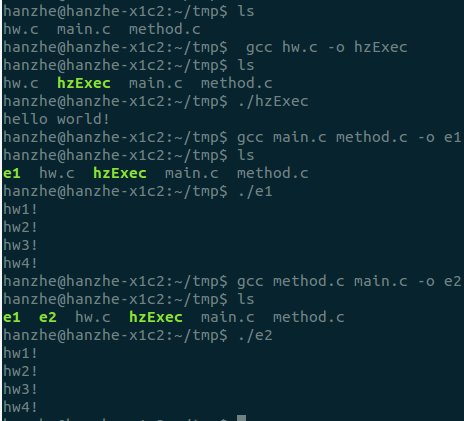
\includegraphics[width=1\linewidth]{ubuntu-gcc-demo.png}

   
  \end{columns}

\end{frame}


\frame{
  \begin{center}
   \Large 谢谢大家!
  \end{center}

}

\end{document}

